% !TEX TS-program = pdflatex
% !TEX encoding = UTF-8 Unicode

% This is a simple template for a LaTeX document using the "article" class.
% See "book", "report", "letter" for other types of document.

\documentclass[hidelinks, 12pt]{article} % use larger type; default would be 10pt
\linespread{1.5} 
\usepackage[utf8]{inputenc} % set input encoding (not needed with XeLaTeX)
\usepackage{amsmath}
\usepackage{pdflscape}
\usepackage{placeins}
\usepackage{hvfloat}


\usepackage{gensymb} %%for degrees C sign

%%%%5FOR COLOR

\usepackage{xcolor}

%%%% IF NOT CAN USE \phantom{} for invisible text


%%% Examples of Article customizations
% These packages are optional, depending whether you want the features they provide.
% See the LaTeX Companion or other references for full information.
\usepackage{textcomp}
\usepackage{amsmath}
\usepackage{array, multirow, bigdelim, makecell, booktabs} 

\usepackage[super]{nth}
\usepackage{amssymb}	
\newcommand\ddfrac[2]{%
    \frac{\displaystyle \raisebox{0.5ex}{$#1$}}%
         {\displaystyle \raisebox{-0.5ex}{$#2$}}%
}

\newcommand\dddfrac[2]{%
    \frac{\displaystyle \raisebox{1ex}{$#1$}}%
         {\displaystyle \raisebox{-1ex}{$#2$}}%
}

%%% PAGE DIMENSIONS
\usepackage{geometry} % to change the page dimensions
 \geometry{
 a4paper,
 total={170mm,257mm},
 left=20mm,
 top=20mm,
 } % or letterpaper (US) or a5paper or....
% \geometry{margin=2in} % for example, change the margins to 2 inches all round
% \geometry{landscape} % set up the page for landscape
%   read geometry.pdf for detailed page layout information
\usepackage{lscape}
\usepackage{graphicx} % support the \includegraphics command and options
\usepackage{longtable}[=v4.13]
% \usepackage[parfill]{parskip} % Activate to begin paragraphs with an
% empty line rather than an indent

\newcolumntype{C}[1]{>{\centering\arraybackslash}p{#1}}
\usepackage{rotating}
\usepackage{pdfpages}
%%% PACKAGES
\usepackage{booktabs} % for much better looking tables
\usepackage{array} % for better arrays (eg matrices) in maths
\usepackage{paralist} % very flexible & customisable lists (eg. enumerate/itemize, etc.)
\usepackage{verbatim} % adds environment for commenting out blocks of text & for better verbatim
%\usepackage{subfig} % make it possible to include more than one captioned figure/table in a single float
% These packages are all incorporated in the memoir class to one degree or another...

\PassOptionsToPackage{hyphens}{url}\usepackage{hyperref}

%%% HEADERS & FOOTERS
\usepackage{fancyhdr} % This should be set AFTER setting up the page geometry
\pagestyle{fancy}
\fancyhf{} % clear all header and footer fields
\fancyfoot[C]{\thepage} % page number in the center of the footer % options: empty , plain , fancy
\renewcommand{\headrulewidth}{0pt} % customise the layout...
\lhead{}\chead{}\rhead{}
\lfoot{}\cfoot{\thepage}\rfoot{}


\fancypagestyle{lscape}{%
\fancyhf{} % Clear all header and footer fields

\fancyfootoffset[R]{-50cm} % Adjust the offset to position the number higher up
\fancyfoot[R]{\makebox[0pt][r]{\rotatebox{90}{\thepage}}} % Page number at bottom right
\renewcommand{\headrulewidth}{0pt}
\renewcommand{\footrulewidth}{0pt}}
%%% SECTION TITLE APPEARANCE
\usepackage{sectsty}
%\allsectionsfont{\sffamily\mdseries\upshape} % (See the fntguide.pdf for font help)
% (This matches ConTeXt defaults)

	
\newcommand{\bsk}{\vspace{\baselineskip}}
\usepackage{float}
%%% ToC (table of contents) APPEARANCE
\usepackage[nottoc,notlof,notlot]{tocbibind} % Put the bibliography in the ToC
\usepackage[titles,subfigure]{tocloft} % Alter the style of the Table of Contents
%%	
%%

\counterwithin{figure}{section}
%%%% modifying toc fonts so they are conssitent
\usepackage{titletoc}
\titlecontents{section}[1em]{\ttfamily}{\thecontentslabel\enspace}{\contentslabel{1em}}{\titlerule*[1pc]{.}\quad\contentspage}[\vskip 4pt]

\usepackage{soul}

%%%%%making a line which is only x cm long
\newcommand{\myline}{\par\noindent\makebox[\linewidth]{\hspace*{-0.4\textwidth}\rule{0.6\textwidth}{0.4pt}}}

%%%%


%\renewcommand\cftchapafterpnum{\vskip6pt}
%\renewcommand\cftsecafterpnum{\vskip6pt}
%\renewcommand\cftsubsecafterpnum{\vskip6pt}
% 
%\renewcommand{\cftchapfont}{\sffamily}
%{\sffamily\tableofcontents}
%\renewcommand{\cftsecfont}{\sffamily}
%\renewcommand{\cftsubsecfont}{\sffamily}
%%%%%

%\renewcommand*\ttdefault{cmvtt}
%\renewcommand*\familydefault{\ttdefault} %% Only if the base font of the document is to be typewriter style
\usepackage[OT1]{fontenc}

%%% END Article customizations
%Structure you want:
%CHP 1
%• Geography - sample sites, a location map, why we went there - a diagram of the Berre? More likely the oyster farming
%• Geology
%• Weather - Ed models
%• Conditions
%• Chemistry
%	◦ Piper diagram is good
%	◦ PHREEQC is good for cations you would expect depending on the composition you have
\usepackage{upgreek}
%CHP 2
%• Describe your data
%• Metals are good
%• Plot on latitude and longitude
%• And colour code for type
%%% The "real" document content comes below...
\usepackage{sectsty}

%\sectionfont{\bfseries\sffamily}
%\subsectionfont{\bfseries\sffamily}
%\subsubsectionfont{\bfseries\sffamily}


%%% remove blank pages
% \let\cleardoublepage=\clearpage 

\setcounter{secnumdepth}{4} % Allow numbering up to 4 levels deep
\setcounter{tocdepth}{4}    % Include up to 4 levels in the Table of Contents

\newcommand{\subsubsubsection}[1]{\paragraph{#1}\mbox{}}

\usepackage{hyperref}
%\usepackage{mathptmx} % Loads a Times-like font for text and math
%\usepackage{newtxtext} % Alternative with a similar appearance
\usepackage[sfdefault]{cabin}
\usepackage[T1]{fontenc}


% Customize the table of contents font to use typewriter style
\titlecontents{section}[1em]{}{}{}{\titlerule*[1pc]{.}\quad\contentspage}
\titlecontents{subsection}[2em]{}{}{}{\titlerule*[1pc]{.}\quad\contentspage}
\titlecontents{subsubsection}[3em]{}{}{}{\titlerule*[1pc]{.}\quad\contentspage}
\titlecontents{paragraph}[4em]{}{}{}{\titlerule*[1pc]{.}\quad\contentspage}


%\renewcommand*\familydefault{\sfdefault} % Uncomment this if you want the entire document in sans-serif






\title{
\vspace{-1cm}
\textbf{Carbon consumption from major mountain belts: \\ The geochemistry of Himalayan groundwaters}

\vspace{0.5cm}



% \begin{figure}[h]
% 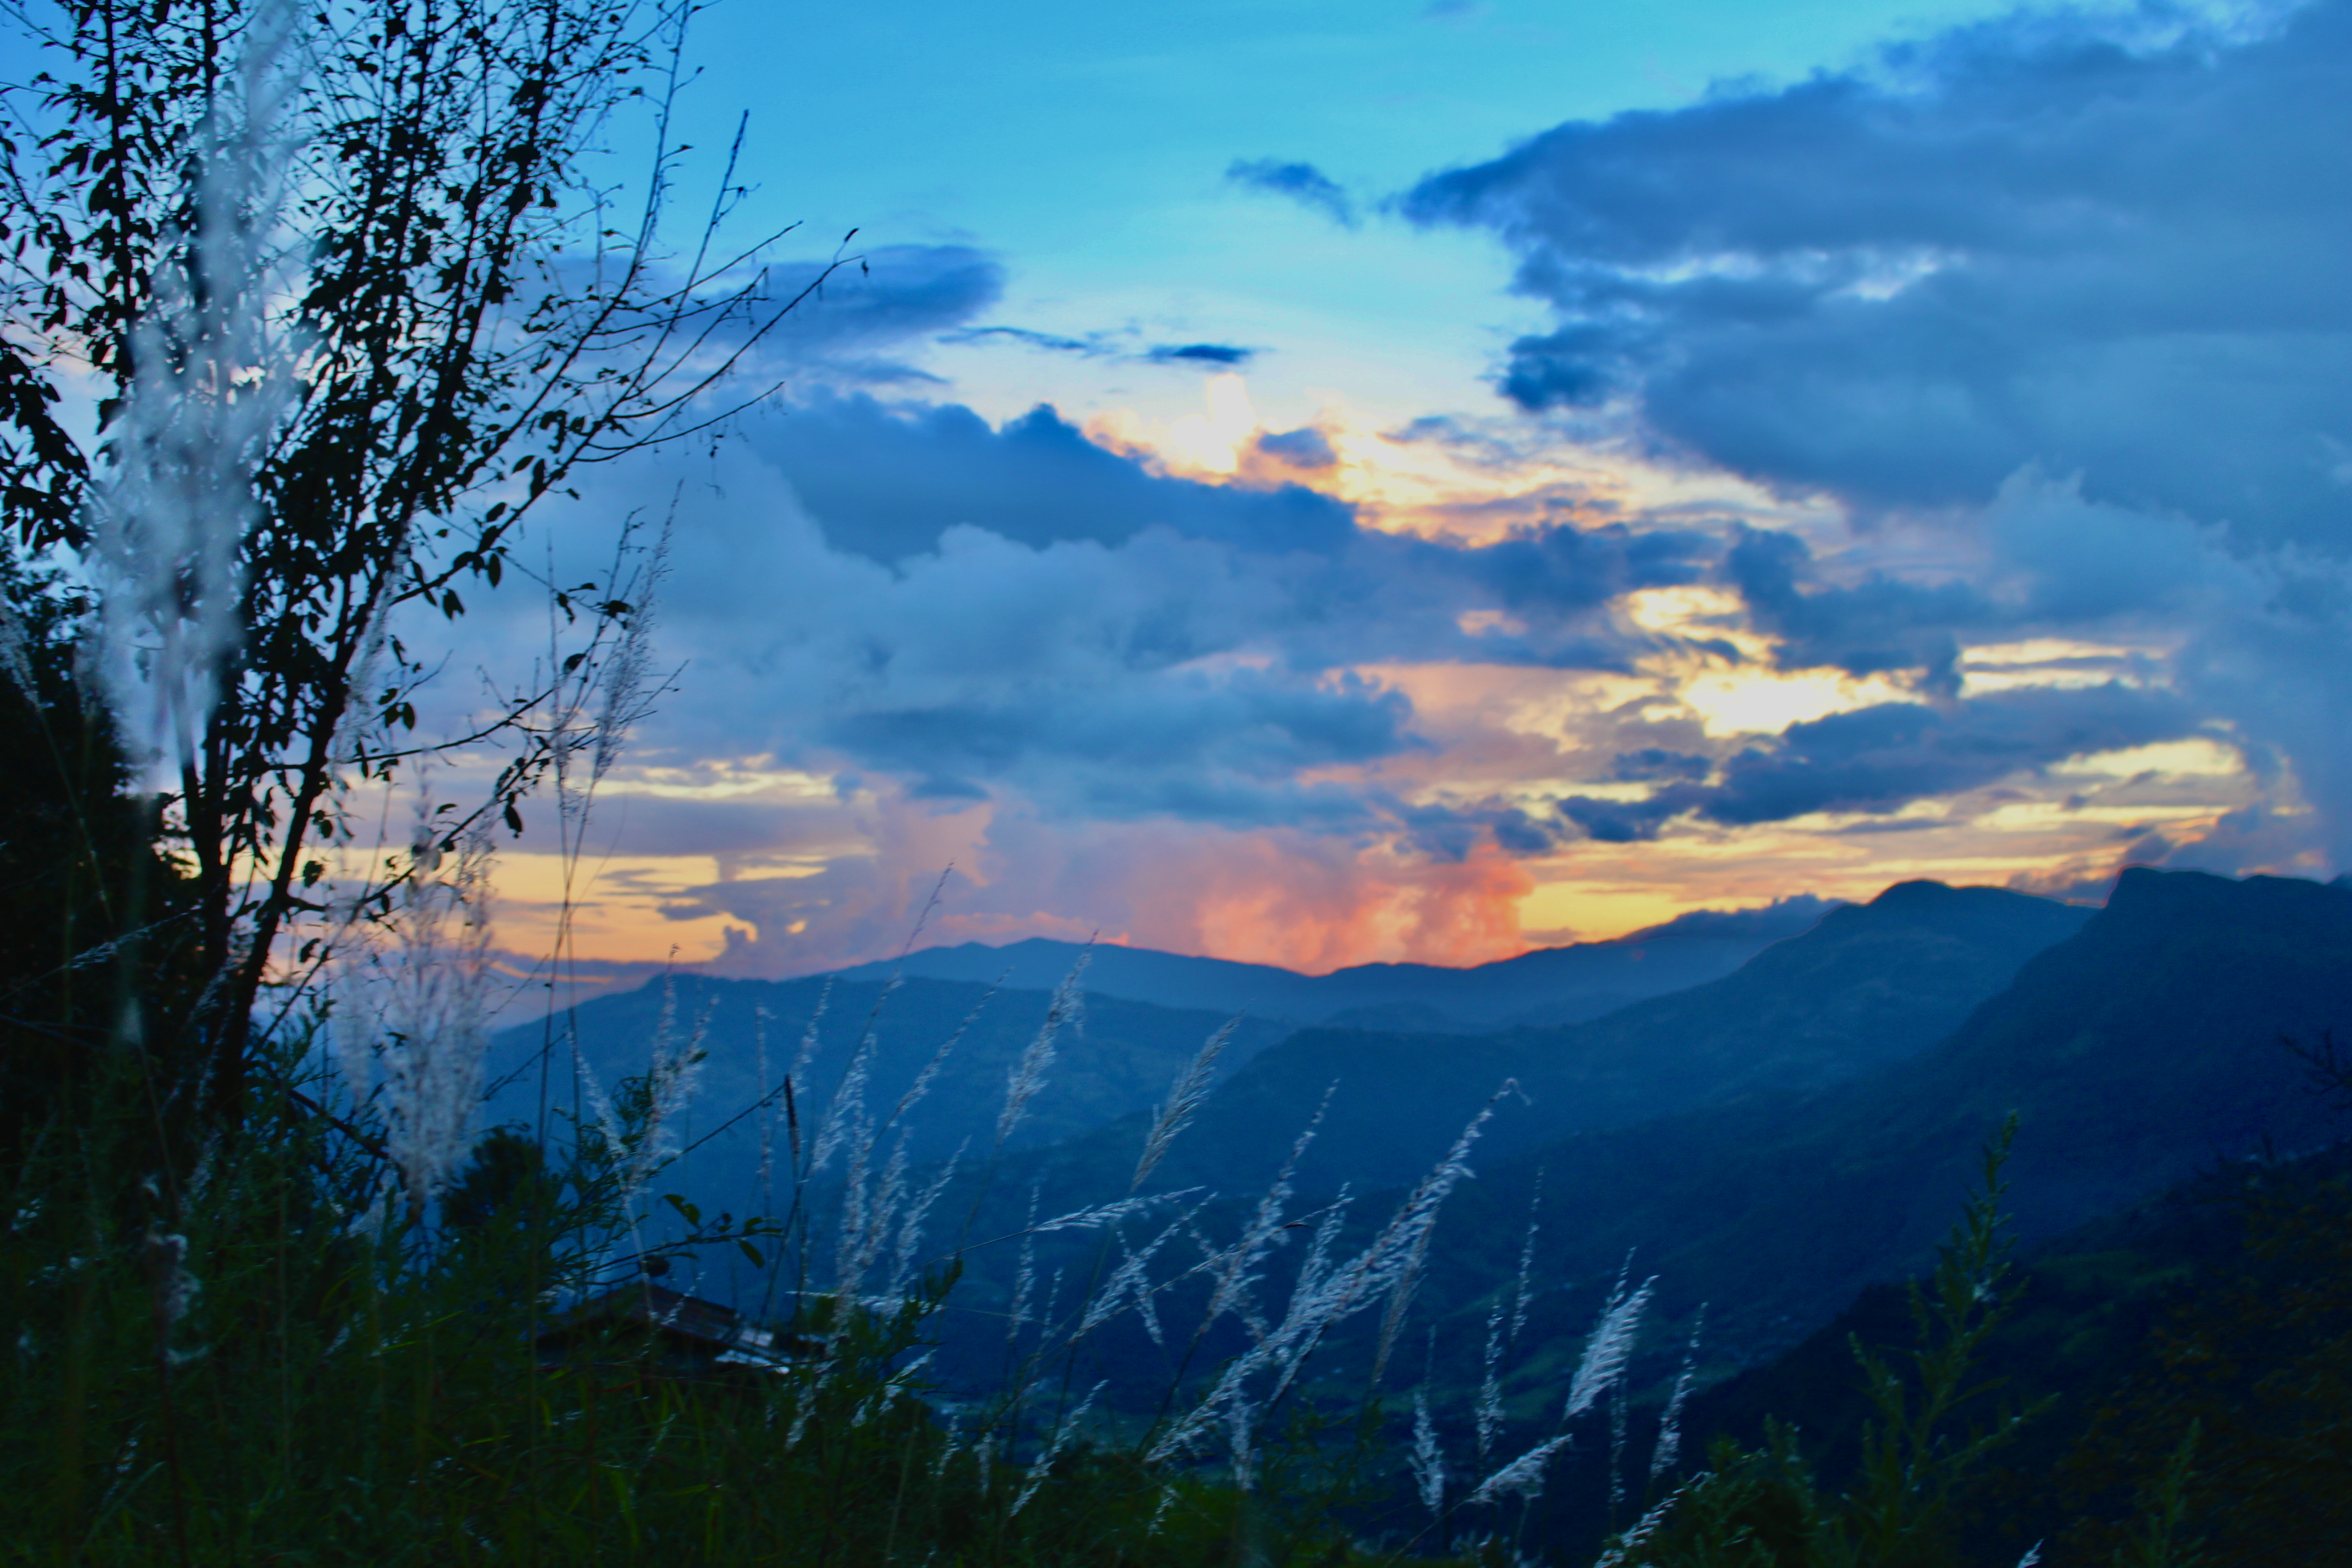
\includegraphics[scale=0.08]{front2.png}
% \centering

% \end{figure}


% University of Cambridge \\
% Part III Project Report \\

% \begin{figure}
%     \centering
%     \begin{subfigure}{.45\textwidth} % Adjust width to leave space between figures
%         \centering
%         \includegraphics[height=4.5cm]{girton.png} % Set the height of the image
%         %\caption{A subfigure}
%         \label{fig:sub1}
%     \end{subfigure}%
%     \hspace{1.5cm} % Add horizontal space between the figures
%     \begin{subfigure}{.45\textwidth} % Adjust width to leave space between figures
%         \centering
%         \includegraphics[height=4.5cm]{cambridge.png} % Set the height of the image
%         %\caption{A subfigure}
%         \label{fig:sub2}
%     \end{subfigure}
%     %\caption{A figure with two subfigures}
%     \label{fig:test}
% \end{figure}


}
\author{Giovanni Bernardi}
\date{2024-2025} % Activate to display a given date or no date (if empty),
         % otherwise the current date is printed 







\begin{document}
\maketitle




\thispagestyle{empty}

\newpage

\section*{Abstract}
\label{sec:abstract}
\addcontentsline{toc}{section}{\nameref{sec:abstract}}

This is the abstract. Feel free to add anything insightful... or not :).


\pagenumbering{roman}

\newpage


\thispagestyle{empty}
%need to change this to the main report font

\tableofcontents
%\thispagestyle{empty}

\newpage

\pagenumbering{arabic}



\FloatBarrier
\pagenumbering{arabic}


\section{Introduction}

Silicate weathering, whereby silicate minerals are dissolved by carbonic acid, 
sequesters atmospheric CO$_2$ over long (10$^6$ year) timescales, influencing global climate regulation. As water passes through the subsurface, it interacts with the surrounding rock. This causes the addition of solute species to the groundwater, and the formation of stable secondary minerals through the dissolution of primary minerals formed at different pressure and temperature. The Himalayan mountain range spans more than 590,000 km$^2$, and is the source of major rivers, including the Ganges, Brahmaputra, and Indus. It is therefore a key region for understanding the global carbon cycle. In highly erosive regions where the supply of silicate minerals far exceeds the weathering rate, silicate weathering reactions are thought to be sensitive to climate. These are regions are called "kinetically-limited" (Stallard \& Edmund 1983 JGR, West et al, 2005) The dissolution kinetics of the silicate rocks in these catchments are thought to be sensitive to temperature and runoff because the weathering reactions have not gone to completion. Silicate weathering in the Himalayas as a result of their uplift and erosion in the Cenozoic may have contributed significantly to the global cooling over the past 40 million years (Raymo and Ruddiman, 1992; West et al, 2005, Kump et al, 2000 Ann Rev Earth Sci). Thus, it is this reported sensitivity to climate as well as their large size that makes them important to study. Models built on this sensitivity ("Fontorbe models" from now on) are used to simulate groundwater through one-dimensional flow paths based on a few key parameters, which make up the "weathering fingerprint" of a catchment (Fontorbe et al., 2013). More recent models have proposed silicate weathering is more sensitive to the hydrological cycle, than to temperature (Maher, 2011). The underlying assumption in these ("Maher models" from now on) is that all weathering paths approach equilibrium. If equilibrium is indeed approached in a particular catchment, then the Maher model is more suitable for use.

\bsk

The weathering fingerprints of these catchments contain many unknowns, namely the residence time of the water, flow path direction and length, rate of reaction, and extent to which equilibrium is reached. Understanding residence time in particular is important because the geochemical and biogeochemical reactions that are used to quantify weathering are time-dependent; longer residence times promote greater solute accumulation in the water (Berner, 1978). These geochemical reactions are also controlled by the reaction rate which is thought to vary as equilibrium is approached (White and Brantley, 2003; Maher, 2011). Therefore, an understanding of residence time will provide insight into how long weathering reactions take place in a given catchment, whether they reach equilibrium, and what this means for the carbon cycle as a whole. Residence time will also reflect the variety of flow routes within a catchment because of physical constraints like Darcy's law, which will help to improve hydrological models. The aim of this study is to compare the Fontorbe and Maher models and their estimation of residence time, and assess their applicability to a real-world catchment.

\bsk

From the model comparison will come a better understanding of fluid residence times in Himalayan catchments, for which tracer data is already commonly used to infer how long a water packet spends in the subsurface (Atwood et al, 2021). Previous studies on Melamchi have used CFC and SF$_6$ gases to determine a mean age on the order of ten years for groundwater at the base of the catchment ridge (Atwood et al, 2021). Using the chemical composition of the water will provide a different way of obtaining residence times, and give a benchmark for the tracer data, which is often reported to be limited in its application (McCallum et al, 2015). If the residence time of a particular water packet is long enough, the reaction will reach chemical equilibrium, meaning the free energy of the system will be close to zero. Comparison of these residence times with estimates of free energy derived from the measured concentration of springwater in the catchment will provide a test on the validity of the two models and their assumptions.

\bsk

The rate of weathering is dependent on the mineralogy of the rock. Different minerals weather at different rates: quartz > albite > mafic silicates > anorthite > carbonates. Therefore, the most reactive minerals will contribute disprportionately to the solute load of the water (Shand et al, 1999). In the Melamchi catchment, only weathering through carbonic acid is considered. Weathering through sulfuric acid is also a big player in the global weathering budget, but its impact is not considered in this study because the marine deposits required for its formation are not present in the Melamchi region (Bufe et al., 2021). Differences in lithology are thought to affect weathering. Geological differences lead to differences in soil composition, landscape features, vegetation, and climate which in turn affect the rates of reaction. Logically, the contribution of one lithology to weathering is correlated to its spatial extent in the catchment (Stallard and Edmond, 1983). Porosities vary widely across a catchment depending on the rock type encountered (Singh et al, 1987; David et al, 1994). Porosity also increases as a rock becomes more weathered (Marques et al, 2009). Weathering regimes can be classified as either transport-limited or kinetically limited (West et al., 2005). West et al. (2005) distinguish the two regimes by the rate of erosion in the catchment. In low erosion rate settings, weathering is transport-limited due to limited mineral supply. Weathering here is therefore proportional to the material eroded. In high erosion rate settings, weathering is kinetically-limited due to an abundant mineral supply. Rapidly eroding catchments like Melamchi are therefore likely kinetically-limited. Soil properties and topography are used to identify different "weathering regimes" in the subsurface (Pedrazas et al, 2021). Indeed, bedrock strength is thought to be more dependent on weathering than mineral or textural differences between the metamorphic lithologies in the Himalayas (Medwedeff et al, 2021). Understanding the extent of weathering can therefore serve to predict the stability of bedrock in rapidly eroding regions. 

\bsk

The strontium isotope composition of different rock types is indicative of different formation mechanisms and conditions. This is used to track the relative contributions of weathering and hydrothermal circulation inputs in seawater (Edmond, 1992). The rock signature imparts a strontium isotopic composition to groundwater that reacts with it in the subsurface. Hence, measuring the strontium isotopic composition of groundwater can provide information on provenance and mixing between streams that react with different lithologies (Faure, 2001).

\bsk

Rates of reaction during weathering comprise both dissolution and precipitation, and chemical equilibrium is defined as that state where these are balanced and equal. Rates of reaction are thought to be different depending on whether they are measured in the field or in a laboratory (Maher et al., 2009). This difference has been explained by denoting 'extrinsic' qualities that are variable in the field, such as permeability and mineral/fluid ratios (White and Brantley, 2003). The rate of reaction of a system has also been linked to the free energy of the system, with laboratory rates being calculated significantly further away from equilibrium than field rates (Kampman et al, 2009). This implies that field localities are closer to equilibrium than laboratory-derived rates might suggest. 

\bsk

The Indian Summer Monsoon (ISM) in Nepal is characterised by a strong seasonal reversal of winds, which brings heavy rainfall to the region during the summer months, and dry conditions during the winter (Bookhagen and Burbank, 2010). The monsoon brings a large amount of precipitation to the region. Oxygen isotopes suggest most of the precipitation occurs in the higher elevation parts of the catchment, and this is supported by remotely sensed rainfall estimates in the region (Acharya et al, 2020; Bookhagen and Burbank, 2010). Precipitation and discharge relationships in the Himalayas have been used to suggest that there is a three month lag in the response of the river to precipitation (Andermann et al., 2012). The residence time of groundwater can be used to quantify this delay and nature of its origin, given that rain is the main source of recharge to the groundwater system (Illien et al, 2021). Studying small catchments gives the opportunity to attribute large changes in water chemistry to seasonal climate changes like the monsoon (Tipper et al., 2006).  Seasonal variation in rainfall is thought to relate to different hydrological regimes, whereby river discharge and precipitation are 'coupled' when there is a significant enough amount of water to recharge the groundwater system. (Illien et al, 2021) The seasonal variation in precipitation therefore also translates to a variation in runoff, whereby this is twelve times stronger during the monsoon than during the dry season (Sharma, 1997). 

\bsk

Changes in climate contribute to changes in the monsoonal system dynamics. The start of the monsoon has not changed in Nepal, but the end has been delayed. This has led to more intense precipitation on a per day basis, which is detrimental for crops in the winter season due to lack of moisture. Intense precipitation is also considered the main climatic cause of flooding (Panthi et al, 2015; Baniya et al, 2012). "One-off" landslide events transport as much as four times the flux of sediment deposited in the valley in a year (Chen C et al., 2023). These events are thought to be increasing in frequency over recent years as a result of climate change, increasing the erosion rate in these areas (Adhikari et al, 2023). In particular, effects of a flash flood in 2021 are still visible in the area, with damage done to several bridges and hundreds of families. 

\bsk

In this study, spring and rain samples from the Melamchi region of Nepal are used as a case study to investigate the weathering rates in a kinetically-limited catchment.
%% LINK TO MAP
The sample dataset consists of 372 samples spanning four field campaigns over three years (2021-2024), as well as more recent year-long bi-weekly timeseries data from stream and spring samples in sites across the catchment. Of those, 68 were collected in September 2024 for this study. This dataset comprises major ion concentrations, alkalinity, and radiogenic strontium isotopes from the Melamchi catchment. 


% \newpage

% \section{Literature Review}

% \subsection{Defining Weathering}

% As water passes through the subsurface, it interacts with rock. This causes the addition of solute species to water, and the formation of stable secondary minerals through the dissolution of primary minerals formed at different pressure and temperature. Dissolved CO$_2$ derived from the atmosphere present in rainfall makes it slightly acidic:\\
% \begin{equation}
% H_2O + CO_2 \rightarrow H_2CO_3 \rightarrow HCO_3^- + H^+
% \end{equation}\\
% Once the rainfall enters the soil as groundwater, the acidicity is further increased by the presence of decomposition of organic matter, and CO$_2$ production from organic activity in the soil.

% \bsk

% The rate of weathering is dependent on the mineralogy of the rock. Different minerals weather at different rates: quartz > albite > mafic silicates > anorthite > carbonates. Therefore, the most reactive minerals will contribute disprportionately to the solute load of the water (Shand et al, 1999). In the Melamchi catchment, only the weathering of carbonic acid is considered. Sulfuric acid is also often considered a big player in weathering, but its impact is not considered in this study because the pyrite deposits required for its formation are not present in lithological studies of the Melamchi region.

% \newpage

% \begin{tcolorbox}[
%     colback=customcolor, % Use the defined custom color for background
%     colframe=white,      % Set the frame color to white (invisible)
%     sharp corners,       % Straight edges
%     boxrule=0pt,         % No border width
%     breakable,           % Allow the box to break into multiple pages (if needed)
%     width=\dimexpr\textwidth+2cm\relax, % Make the box wider than \textwidth
%     enlarge left by=-1cm,   % Shift box left to center the extra width
%     leftrule=0mm,        % No left border
%     rightrule=0mm,       % No right border
%     toprule=0mm,         % No top border
%     bottomrule=0mm       % No bottom border
% ]
% \textbf{\Large Box 1: Chemical Weathering Reactions}
% \vspace{-3mm}
% \myline\\
% {\footnotesize
% Chemical weathering reactions are dependent on the lithology and acid content of the water. Below are the primary reactions that characterise carbonic acid weathering worldwide.

% \bsk

% \textbf{Carbonic Acid Weathering of Carbonate}\\
% This reaction has no effect on atmospheric CO$_2$ levels in the long term.

%     \begin{center}
    
%     Short Term (10$^3$ years):
%     \begin{equation}
%     CaCO_3 + CO_2 + H_2O \rightarrow Ca^{2+} + 2HCO_3^-
%     \end{equation}
    
%     Long Term (10$^6$ years):
%     \begin{equation}
%     Ca^{2+} + 2HCO_3^- \rightarrow CaCO_3 + CO_2 + H_2O
%     \end{equation}

%     \end{center}
    
    
% \textbf{Carbonic Acid Weathering of Silicate}\\ This produces net CO$\ttmath{_2}$ drawdown. Reactions are written for a generic Ca-rich plagioclase mineral.

%     \begin{center}

%     Short Term (10$^3$ years):
%     \begin{equation}
%     2CO_2 + 3H_2O + CaAl_2Si_2O_8 \rightarrow Ca^{2+} + 2HCO_3^- + Al_2Si_2O_5(OH)_4
%     \end{equation}
    
%     Long Term (10$^7$ years):
%     \begin{equation}
%     \ttmath{Ca^{2+} + 2HCO_3^- \rightarrow CaCO_3 + CO_2 + H_2O}
%     \end{equation}
    
%     \end{center}

% }
% \end{tcolorbox}


% \subsection{Geological Controls on Weathering}


% The rate of weathering is dependent on the mineralogy of the rock. Different minerals weather at different rates: quartz > albite > mafic silicates > anorthite > carbonates. Therefore, the most reactive minerals will contribute disprportionately to the solute load of the water (Shand et al, 1999). In the Melamchi catchment, only the weathering of carbonic acid is considered. Weathering of sulfide minearls is also a big player in the global weathering budget, but its impact is not considered in this study because the marine deposits required for its formation are not present in the Melamchi region (Bufe et al., 2021). Differences in lithology are thought to affect weathering. Geological differences lead to differences in soil composition, landscape features, vegetation, and climate which in turn affect the rates of reaction. Logically, the contribution of one lithology to weathering is correlated to its spatial extent in the catchment (Stallard and Edmond, 1983). Porosities vary widely across a catchment depending on the rock type encountered (Singh et al, 1987; David et al, 1994). Porosity also increases as a rock becomes more weathered (Marques et al, 2009). Weathering regimes can be classified as either transport-limited or kinetically limited (West et al., 2005). West et al. distinguish the two regimes by the rate of erosion in the catchment. In low erosion rate settings, weathering is transport-limited due to limited mineral supply. Weathering here is therefore proportional to the material eroded. In high erosion rate settings, weathering is kinetically-limited due to an abundant mineral supply. Rapidly eroding catchments like Melamchi are therefore likely kinetically-limited. Soil properties and topography are used to identify different "weathering regimes" in the subsurface (Pedrazas et al, 2021). Indeed, bedrock strength is thought to be more dependent on weathering than mineral or textural differences between the metamorphic lithologies in the Himalayas (Medwedeff et al, 2021).



% \subsection{Reaction Rates in Natural and Laboratory Settings}

% Rates of reaction during weathering comprise both dissolution and precipitation, and chemical equilibrium is defined as that state where these are balanced and equal. Rates of reaction are thought to be different depending on whether they are measured in the field or in a laboratory (Maher et al., 2009). This difference has been explained by denoting 'extrinsic' qualities that are variable in the field, such as permeability and mineral/fluid ratios (White and Brantley, 2003). The rate of reaction of a system has also been linked to the free energy of the system, with laboratory rates being calculated significantly further away from equilibrium than field rates (Kampman et al, 2009). This implies that field localities are closer to equilibrium than laboratory-derived rates might suggest. 



% \subsection{Response to Monsoonal Precipitation}

% The Indian Summer Monsoon (ISM) is characterised by a strong seasonal reversal of winds, which brings heavy rainfall to the region during the summer months, and dry conditions during the winter (Bookhagen and Burbank, 2010). The monsoon brings a large amount of precipitation to the region. Oxygen isotopes suggest most of the precipitation occurs in the higher elevation parts of the catchment, and this is supported by remotely sensed rainfall estimates in the region (Acharya et al, 2020; Bookhagen and Burbank, 2010). Studying small catchments gives the opportunity to attribute large changes in water chemistry to seasonal climate changes like the monsoon (Tipper et al., 2006).  Seasonal variation in rainfall is thought to relate to different hydrological regimes, whereby river discharge and precipitation are 'coupled' when there is a significant enough amount of water to recharge the groundwater system. (Illien et al, 2021) The seasonal variation in precipitation therefore also translates to a variation in runoff, whereby this is twelve times stronger during the monsoon than during the dry season (Sharma, 1997). 

% \bsk

% Andermann et al. (2012) report anticlockwise hysteresis loops of precipitation against discharge (include figure?), and suggest that there is a three month lag in the response of the river to precipitation.  The delay in river discharge is a topic of debate. Andermann et al. (2012) propose that at lower elevations, it is more likely due to groundwater storage of precipitation in the fractured basement. Bookhagen and Burbank (2010) suggest that the delay of precipitation and discharge may be due to the response of glaciers at higher elevations. They also suggest evaportranspiration has a low impact on the hydrological budget of the Himalayas, less than 10\%. Other studies have found that catchments with little glacial input show the same delay, suggesting that the former hypothesis may be more relevant to this discussion (McGuire et al, 2005). The residence time of groundwater can hence be used to quantify this delay and nature of its origin, given that rain is the main source of recharge to the groundwater system (Illien et al, 2021). 


% \subsection{Effects of a Changing Climate}

% Changes in climate contribute to changes in the monsoonal system dynamics. The start of the monsoon has not changed in Nepal, but the end has been delayed. This has led to more intense precipitation on a per day basis, which is detrimental for crops in the winter season due to lack of moisture. Intense precipitation is also considered the main climatic cause of flooding (Panthi et al, 2015; Baniya et al, 2012). 

% \bsk

% "One-off" landslide events transport as much as four times the flux of sediment deposited in the valley in a year (Chen C et al., 2023). These events are thought to be increasing in frequency over recent years as a result of climate change, increasing the erosion rate in these areas (Adhikari et al, 2023). In particular, effects of a flash flood in 2021 are still visible in the area, with damage done to several bridges and hundreds of families. 



% Summary of the key questions (commented):
% 1. What main challenge does this study address?
% 2. What prior work and prevailing perspectives exist?
% 3. What does this investigation aim to accomplish?
% 4. Which results are highlighted by this study?
% 5. How have previous models approached the problem?
% 6. In what ways does this work differ from existing studies?
% 7. Why is this approach potentially more beneficial?
% 8. Which specific questions does this study seek to answer?











\section{Study Area}
% Provide a description of the sampling methods, field area, and geology.
% - Include maps or figures if necessary.

% want table with catchment characteristics
% also remember to include a table with abbreviations


The Melamchi-Indrawati catchment (85.441 - 85.601 E, 27.822 - 28.157 N) study area ranges from 790 to 5700 m a.s.l. (metres above sea level). The Melamchi River is a tributary of the larger Indrawati River and runs through the catchment draining an area of 325km$\ttmath{^2}$. 

\subsection{Geology and Geomorphic setting}

% Need to add Himalayan background

The geology of Melamchi is characterised by the characteristic banded gneiss, feldspathic schist and laminated quartzite of the Higher Himalayan Crystalline Sequence (HHCS). To the south of the confluence of the Melamchi River to its parent Indrawati river lies the Main Central Thrust (MCT) which separates the HHCS from the Lower Himalayan Sequence (LHS) (Dhital et al, Graf et al). The overall geology is therefore largely comprised of silicate metamorphic rock. (map)

\subsection{Climate}

Annual mean temperatures in the Melamchi Khola Catchment range from ~24$^{\circ}$C at base elevation to ~8$^{\circ}$C at highest elevation sampled (3200 m a.s.l.). The area is characterised by a high erosion rate.  The southern Himalayas are characterised by a large topographic gradient. This corresponds to a large temperature gradient contributing to tropical and alpine climates close to one another (Kattel et al, 2012). The westerly winds typical of this latitude are responsible for the dry season in the Himalayas (Bookhagen and Burbank, 2010). The source of precipitation during the Indian Summer Monsoon (ISM) affecting Melamchi is the Bay of Bengal, due to the strong pressure gradient that changes the westerly winds to southerly winds. This temperature gradient reverses in the winter, when the oceans are warm and the High Himalaya is cold.  The Melamchi Khola catchment receives over 80\% of its rainfall during the monsoon.





% \begin{itemize}

% \item{What is the lat long extent of the study area?}

% 85.441 - 85.601 E, 27.822 - 28.157 N

% \item{What is the elevation range of the catchment?}

% 786 - 5697m

% \item{What is the area that the river drains? How do you calculate that (i.e. DEM)?}

% 325 km$^2$

% \item{What is the geology of the area?}



% \item{What is the climate of the area? what is it influenced by? i.e. monsoon, etc.}

% Bookhagen and Burbank (2010) identify two main climatic influences in the Himalayas: the monsoon system and the westerlies. The westerly winds, typical of this latitude, are responsible for the dry season in the Himalayas. The system is further divided into the East Asian and Indian Monsoon systems, which interact with each other. The high elevation of the High Himalayas creates a barrier that affects atmospheric circulation.  Bookhagen et al. (2005b) suggest that the Tibetan Plateau's high elevation generates a low-pressure cell near the surface, altering atmospheric circulation patterns.  This is one explanation for the monsoon, though other studies present differing views (see Bookhagen and Burbank, 2010 for a discussion). The source of precipitation during the Indian Summer Monsoon (ISM) affecting Melamchi is the Bay of Bengal, due to the strong pressure gradient that changes the westerly winds to southerly winds. This temperature gradient reverses in the winter, when the oceans are warm and the High Himalaya is cold.


% The high elevation of the High Himalayas creates a barrier that affects atmospheric circulation.  Bookhagen et al. (2005b) suggest that the Tibetan Plateau's high elevation generates a low-pressure cell near the surface, altering atmospheric circulation patterns.  This is one explanation for the monsoon, though other studies present differing views (see Bookhagen and Burbank, 2010 for a discussion). 


% Factor of 12 variation in runoff Tipper et al, 2006 and Sharma 1997


% \item{What is past literature on rainfall in monsoon season?}

% \item{What about clouds and fog? Especially when you are here?}

% \item{What are the annual mean temperatures at different elevations?}

% 24C at base elevation, ~900masl and 8C at highest elevation, ~3200masl.

% \item{What is the lapse rate like?}

% \item{What is the vegetation like?}

% Veget


% \item{Make sure to insert a description of the catchment: catchment, Area, mean slope, mean elevation, elevation range, land cover type, geology, Lat Long range}

\begin{table}[h!]
\centering
\begin{small}
\begin{tabular}{p{3cm} p{1cm} p{1cm} p{1.8cm} p{1.9cm} p{1.5cm} p{3cm}}
       \hline
       \textbf{Catchment} & \textbf{Area} & \textbf{Mean Slope} & \textbf{Mean Elevation} & \textbf{Elevation Range} & \textbf{Geology} & \textbf{Location Range (DD)} \\[4pt]
                          & (km$^2$)    & (\%)                & (m)                     & (m)                      &                &  \\[4pt]
       \hline
       Melamchi Khola     & 325         & 20                  & 2400                    & 786--5697                & HHCS           & 85.441--85.601 E  27.822--28.157 N \\[4pt]
       \hline
\end{tabular}
\end{small}
\caption{Catchment characteristics of the study area.}
\label{tab:catchment_characteristics}
\end{table}


% elevation range from DEM
% area from DEM, and software to figure out catchment area

% \end{itemize}



\section{Data collection and analysis}
% Discuss the analytical methods used in the study.
% - Refer to relevant data tables.



\subsection{Field Sampling}
Two types of water body were sampled in the field: springs and rain. Springs were sampled from the closest identified source in
 the study area, and rain was collected in a rain gauge.
Both were measured in the field for temperature, pH and TDS on a Hanna Instruments HI-991300 and  and EXTECH DO700. The field measurements 
were done at the source for the springs, and back at base for the rain before titrating, 
24 hours within having been collected. 
Six aliquots were collected for each spring for anion, cation, titration, DIC, isotope and archive purposes respectively. 
Rain samples had a smaller yield and so only three aliquots were collected, for ion, isotope and archive purposes. 
Both water body types were filtered through a 0.2µm PES membrane in a filtration unit prior to bottling. 
Cation and archive samples were acidified with concentrated HNO$_3$ to give a pH of $\sim$2, keeping the cations in solution. 
Samples were titrated with a Hach digital titrator with 0.0625M HCl to calculate the alkalinity of the water following the Gran Method (Gran, 1952).



%Titration uncertainty!! Use the mean square error of the titration to calculate the uncertainty of the alkalinity.



\subsection{Major and Trace Element Analysis}

Ion concentrations were measured in Cambridge once back from the field. Cation concentrations were determined using a Agilent Technologies 
5100 Inductively-Coupled Plasma Optical Emission Spectrometer (ICP-OES) using a calibration line made from a Nepalese spring stock solution.
Anion concentrations were determined using a Dionex ICS-5000 Ion Chromatograph against the Battle-02 standard calibration line. Associated 
uncertainties range between 5-10\% for cations and 10-15\% for anions.

%fact check the anion uncertainty

\subsection{Sr Isotope Analysis}

Samples were dried down to provide at least 1 $\mu$g of Sr. Samples were then dissolved in aqua regia (3:1 HNO$_3$:HCl) to remove any additional organic matter. Once dried down again, they were added to 30 $\mu$l teflon columns with Eichrom SrSpec$^{\textcopyright}$ resin pipetted in. Once washing the column three times with Milli-Q$^{\textregistered}$ water, it was primed with 3N HNO$_3$. The sample was centrifuged then loaded onto the column avoiding any solids. The column was then washed a total of three times with 3N HNO$_3$ to remove cations. Lastly the column was eluted to a beaker with Milli-Q$^{\textregistered}$ water to collect the Sr. Once dried, the samples were ...





\subsection{Cyclic and hydrothermal Correction + radiogenic?}

Rain input is a significant factor in the chemical composition of rivers (Drever, 1997).
Spring water is corrected for rain input according to the average concentration for the closest 
rain sample collected in this field season. % can remove if too much text

\bsk

To remove the contribution of the rain the following formula is used for any element X:

\begin{center}
{\Large
$[X]_{rain-corrected}$  = $[X]_{river}$ - $(Cl_{river} - Cl^*_{river})\ddfrac{[X]_{rain}}{[Cl]_{rain}}$}

\end{center}

Where $[Cl]^*_{river}$ is is calculated by subtracting the concentration of chloride in the rain from that in the river (Tipper et al, 2006).
$Cl^{*}$ is taken to be zero if the concentration of chloride in the rain is greater than concentration of river. Evapotranspiration is not considered by this model, because of
studies like Andermann et al (2012) which show that it plays a minor role, accounting for less than 10\% of the hydrological budget in the Himalayas.
They agree with Bookhagen and Burbank


%do we keep this??

\bsk
\bsk

% {\tiny
% This formula is used because it allows for evapotranspiration to be corrected for in a later revision. 

% Evapotranspiration (ET henceforth) is a term that describes the sum of evaporation and plant transpiration 
% from the earth's land surface to atmosphere, including soil and vegetation.[Cite]. 
% ET is crop dependent and intuitively varies as rainfall with time. ET is calculated 
% using the Penman-Monteith method, and there exists literature which compile global 
% annual databases of ET. These can be compared for the Cañete to rainfall, and the above equation can be modified like so:

% \begin{center}
% {\Large
% $[X]_{rain-corrected}$ = $[X]_{river}$ - $\frac{[X]_{rain}}{[Cl]_{rain}} *[Cl]_{lowest-river}  * ETF   $}

% \end{center}

% Where ETF is an evapotranspiration factor relating the relative amonts of rain to evapotranspiration. 
% For example,  if half the rain gets evaporated, then the samples will be more concentrated when corrected (and the minimum ET is zero).
% }
\bsk
\bsk


In those cases where $Cl^*$ is not zero then, a primary rain correction is simply:


\begin{center}
{\Large
$[X]_{rain-corrected}$  = $[X]_{river}$ - $[X]_{rain}$}

\end{center}

\bsk

Once the samples have been corrected for rain input, the remaining $[Cl]^{-}$ is assumed to be derived from evaporites encountered in the flow path. 

% Do we do this?
Hence, the sample with the highest $[Cl]^{-}$ is used to correct the ions in a similar fashion to how the most dilute sample was used above:

\begin{center}
{\Large
$[X]_{evaporite-corrected}$  = $[X]_{rain-corrected}$ - $\frac{[X]}{[Cl]}_{highest-Cl} * [Cl]_{rain-corrected}$}
\end{center}

This ensures that all chloride in the corrected sample is removed. 
The correction uses ionic ratios from the most concentrated water source, 
which acts as a proxy for the sediment imparting its signature. 
In this way, the correction does not affect samples which do not have high Cl 
(and hence do not have a large evaporite contribution), but does decrease the concentration of ions for those that do.

\bsk

% As a further detail when modeling a groundwater flow, 
% it is unlikely that the composition of Sample$_{highest-Cl}$ is just a product of evaporites. 
% The water will also flow over silicate and carbonate rocks. 
% Under the assumption that the evaporite in question is stoichiometric halite, 
% any additional sodium in the Na:Cl ratio of Sample$_{highest-Cl}$ comes from 
% silicate weathering (primary silicate weathering, if you will). 
% Quantifying the effect of this primary weathering is highly complicated 
% and a topic worthy of its own investigation (eg my part III project). 
% However, it can be to a first approximation factored out if all of the ratios 
% are normalised such that Na:Cl is equal to 1 (i.e. divide each ratio by Na:Cl for Sample$_{highest-Cl}$).

%\subsection{Evapotranspiration Estimates}
%???






\section{Seasonal and Spatial Variation}

\subsection{Springs changing concentration with season, indicating monsoonal precipitation influence}
\textcolor{red}{Systematic undulation september to october to november to april. Small amount compared to rainfall Si...} Several springs show evidence for a concentration decrease during the monsoon, as increased water flux dilutes the normal element load in the water. This is also visible in a spring time series over several months. Both sample sets display a decrease in concentration in September, where the effect of the monsoon is the greatest. It would be worth it to compare to previous literature values.??




\begin{figure}[h]
    \centering
    \includegraphics[width=0.8\textwidth]{Si_mM_concentrations_springs.pdf}
    \includegraphics[width=0.8\textwidth]{Si_mM_Thalo_timeseries.pdf}
    \caption{Seasonal changes in spring concentration indicating monsoonal precipitation influence.; Time series of spring concentration changes over time.}
    \label{fig:time_series_changes}
\end{figure}

\FloatBarrier

\bsk

Recorded temperature at the end of the spring flow paths is variable with the season, and is coldest at the end of the monsoon in November. All seasons show a temperature decrease with increasing elevation, suggesting consistent sampling of spring flow paths. 
\textcolor{red}{Spring temperature is close to lapse rate (what ref?)} 


\begin{figure}[h]
    \centering
    \includegraphics[width=\textwidth]{Temperature_Elevation_Season.pdf}
    \caption{Temperature cahnges}
    \label{fig:seasonal_change2}
\end{figure}

\FloatBarrier

\newpage


\subsection{Spatial concentration changes between the springs}

Broadly, the northernmost three traverses display a linear trend of concentration and alkalinity with elevation \textcolor{red}{Alkalinity slightly different...} . The southernmost two traverses display a distinct jump in concentration. This could suggest that the springs sampled tap into different lithologies, but this could also be due to longer flow paths and a closer approach to equilibrium. The possible controls on these variations, namely temperature, flow path length, lithology, dissolution rates, and evapotratnspiration cannot easily be distinguished.

\begin{figure}[h]
    \centering
    \begin{tabular}{c}
        \includegraphics[width=0.8\textwidth]{Si_mM_EC_Elevation.pdf} \\
        \includegraphics[width=0.8\textwidth]{Alkalinity_Elevation.pdf} \\
    \end{tabular}
    \caption{How Alkalinity and Si changes with elevation}
    \label{fig:spatial_changes_spring2}
\end{figure}

\FloatBarrier

% \begin{figure}[h]
%     \centering
%     \includegraphics[width=\textwidth]{SiCaNaCa.pdf}
%     \caption{Si/Ca against Na/Ca. Clear differences between traverses.}
%     \label{fig:spatial_changes_spring3}
% \end{figure}



% \begin{figure}[h]
%     \centering
%     \includegraphics[width=\textwidth]{NaClEl.pdf}
%     \includegraphics[width=\textwidth]{ClEl.pdf}
%     \caption{NaCl against elevation coloured by traverse -  super low Cl; Cl against elevation coloured by traverse - Potential evaporite influence on traverse 2 water chemistry}
%     \label{fig:spatial_changes_spring5}
% \end{figure}

% \FloatBarrier

\newpage


\subsection{Sr isotope against 1/Sr data \textcolor{red}{Change title} }
\textcolor{red}{make this whole subsection simpler} 
Radiogenic strontium isotope analyses of springs similarly show a wide variation between different traverses. Due to the unique source-tracking nature of strontium isotopes this is potentially explained with varying lithology along the ridge. These variations are however consistent with the range of Higher Himalayan Crystalline Series (HHCS) rocks found in the region (Tipper et al., 2006), so it is unlikely that the source of the Sr isotopes is from the Lesser Himalayan Series (LHS) rocks - the MCT is quite a bit more south than this \textcolor{red}{Make this sentence simpler} .

\bsk

Sr isotopes derived from the most recent rain analyses are of the order of 0.70904 to 0.70925 at the lowest. Seawater is of the order of 0.70917. Within error, therefore, the lowest rain values reflect seawater strontium isotope values, indicating little contamination from dust or particles. The non-contaminated samples are indeed found at the higher elevations, and they show low chloride concentrations consistent with rain. \textcolor{red}{Need a table with errors} 

\bsk

Compared to the springs on a 87Sr/86Sr against 1Sr plot (Figure 5D eg), there is no significant spring mixing line towards the rain. This suggests that the spring water undergoes significant chemical weathering compared to the initial input, suggesting long flow paths and/or long residence times.


\begin{figure}[p]
    \centering
    \includegraphics[width=\textwidth]{Sr87_Sr86_1_Sr.pdf}
    \includegraphics[width=\textwidth]{Sr87_Sr86_Elevation.pdf}
    \caption{Strontium isotope differences display difference in lithology tapped in. Cite Quade and Tipper papers; Rain analysed for Sr isotopes and Cl. Something about contamination lower down; How samples of Traverse 3 compare to the rain samples}
    \label{fig:discussion3}
\end{figure}

\begin{figure}[p]\ContinuedFloat
    \includegraphics[width=\textwidth]{Sr87_Sr86_Cl.pdf}
    \includegraphics[width=\textwidth]{Sr87_Sr86_1Sr_Rain.pdf}
    \caption[]{(Continued)}
\end{figure}

\FloatBarrier

% \begin{figure}[h]
%     \centering
%     \includegraphics[width=\textwidth]{Sr87_Sr86_1Sr_Traverse_Triangle.pdf}
%     \caption{Recreating the Lanord plot etc. Need to choose better endmembers}
%     \label{fig:discussion4}
% \end{figure}

% Also include 87Sr/86Sr weathering according to that mass balance thing... if that helps

\newpage

\subsection{Traverse 3 is the best sampled and least influenced - \textcolor{red}{Need a better title}}

It is difficult to explain the inter-traverse variation in concentration and isotopic composition. As a result, for the remainder of this study's analysis, only Traverse 3 out of the five will be chosen as a case study representing the catchment. Whilst it is also possible that all traverses' flow paths are connected one to the other \textcolor{red}{something about just traverse 3}. This is because, for traverse 3, there is little evidence to suggest lithology is not constant. For one, geological maps suggest lithology does not vary across E-W, which is the profile all traverses follow. Secondly as is evident from the Na/Si against itself plot, Na/Si plots almost exactly on the 1:1 line for every season where the same spring was sampled in Traverse 3. The fact that this ratio increases with decreasing elevation suggests more and more Si is reprecipitated, while Na is only involved in dissolution. The narrow range and tight scatter suggests little lithological change and consistently sampled flow paths over time. This is even more apparent when plotting against elevation for different seasons.

\begin{figure}[p]
    \centering
    \includegraphics[width=0.5\textwidth]{ExampleFlow.pdf}
    \includegraphics[width=\textwidth]{Si_mM_EC_Ridge_Distance.pdf}
    \caption{How Si varies for Traverse 3, showing a wide variety of samples; Na/Si for Traverse 3 is pretty neat. Consistently sampled flow paths.}
    \label{fig:spatial_changes_spring8}
\end{figure}

\begin{figure}[p]\ContinuedFloat
    \centering
    \includegraphics[width=\textwidth]{Na_Si_Trav3.pdf}
    \includegraphics[width=\textwidth]{Na_Si_Elevation.pdf}
    \caption[]{(Continued)}
\end{figure}

\FloatBarrier


% \begin{figure}[h]
%     \centering
%     \includegraphics[width=\textwidth]{Na_Si_Trav3.pdf}
%     \caption{Na/Si for Traverse 3 is pretty neat}
%     \label{fig:spatial_changes_spring9}
% \end{figure}

% \FloatBarrier








\section{Discussion}
% Explain how to interpret the data.
% - Divide the analysis into different geological provinces.
% - Discuss the characteristics of each province.




Andermann et al, 2012

They also talk about a modelLook at response time, being inveresely proportional to hydraulic diffusivity.
THey assume length scales of 0.5-5km, and typical values of time to be about 45 days.

They are looking at very large discharges, order 5000 m3/s




\bsk

Also want the Maher and Chamberlain rate constant explanation compared to normal data

\bsk

Want to input the beginning steps of the derivation from Maher and Chamberlain, 2014's model. Eg the solution to a heterogeneous irreversible advection reaciton equation



\bsk
\[
\ttmath{C = \frac{C_0}{1 + D} + C_{eq} \cdot \frac{D}{1 + D}}
\]
\[
\ttmath{D = \frac{\tau \cdot D_w}{q}}
\]
\[
\ttmath{D_w = \frac{L \cdot \phi}{T_{eq}}}
\]
\[
\ttmath{L = q \cdot t}
\]
\[
\ttmath{T_{eq} = \frac{C_{eq}}{R \cdot f}}
\]
\[
\ttmath{R = \rho \cdot k \cdot A \cdot X}
\]
\[
\ttmath{k = 8.7 \cdot 10^{-6}  \; mol/m^2/yr}
\]
\[
\ttmath{k = 8.7 \; \mu mol/m^2/yr}
\]
\subsection{Step 1: Rearrange for $D$}
Multiply through by $(1 + D)$:
\[
C \cdot (1 + D) = C_0 + C_{eq} \cdot D
\]

Distribute $C$:
\[
C + C \cdot D = C_0 + C_{eq} \cdot D
\]

Group terms involving $D$:
\[
C \cdot D - C_{eq} \cdot D = C_0 - C
\]

Factor $D$:
\[
D \cdot (C - C_{eq}) = C_0 - C
\]

Solve for $D$:
\[
D = \frac{C_0 - C}{C - C_{eq}}
\]

\subsection{Step 2: Solve for $t$ Using $D$}
Now substitute $D$ into:
\[
D = \frac{\tau \cdot t \cdot \phi \cdot R \cdot f}{C_{eq}}
\]

Rearranging for $t$:
\[
t = \frac{D \cdot C_{eq}}{\tau \cdot \phi \cdot R \cdot f}
\]

Substitute $D$:
\[
t = \frac{\left(\frac{C_0 - C}{C - C_{eq}}\right) \cdot C_{eq}}{\tau \cdot \phi \cdot R \cdot f}
\]

Simplify:
\[
t = \frac{(C_0 - C) \cdot C_{eq}}{(C - C_{eq}) \cdot \tau \cdot \phi \cdot R \cdot f}
\]

\subsection{Conclusion}
The expression for $t$ is:
\[
t = \frac{(C_0 - C) \cdot C_{eq}}{(C - C_{eq}) \cdot \tau \cdot \phi \cdot k \cdot M_{in} \cdot f}
\]
Where:
\begin{itemize}
    \item $C_0$: Initial concentration.
    \item $C$: Current concentration.
    \item $C_{eq}$: Equilibrium concentration.
    \item $\tau$: Characteristic timescale.
    \item $\phi$: Porosity.
    \item $R$: Reaction rate term.
    \item $f$: Scaling factor.
\end{itemize}




\input{references.tex}


\end{document}







%%  pdflatex Part3Report.tex && open Part3Report.pdf  